\section{New Design}

The new design greatly simplifies the implementation by reducing integration
points and coupling things where they naturally make sense. The minutiae of
creating, confirming, and releasing jobs doesn't need to be performed by a
scheduler; moving this all to mom daemons allows Moab to do what it does best –
schedule. Mom daemons already manage everything that has to do with setting up
jobs, starting them, and cleaning up after them once completed, so the ALPS
interactions belong on the moms. Finally, having all of the integration a
single daemon reduces integration points, making the code easier to understand
and maintain.

\subsection{How It Works}
\begin{figure}
  \centering
  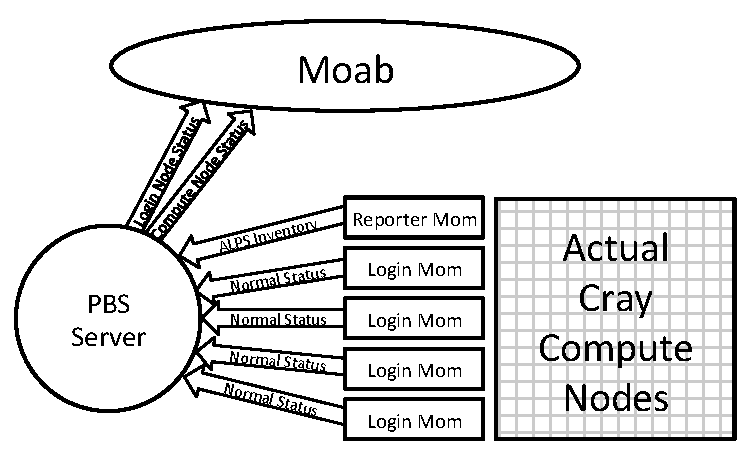
\includegraphics[width=3.6in]{figures/new-diagram.pdf}
  \caption{New Reporting Structure}\label{fig:reporting}
\end{figure}

All ALPS integration now takes place on the mom daemons as shown in Figure
\ref{fig:reporting}. Two different kinds of mom daemons are run for this setup:
a reporter mom and one or more alps_login moms. The reporter mom's only
function is to report the inventory information to pbs_server, which then
discovers all of the computes.

The other mom daemon is the alps_login type, which manages job starts. The
login mom creates and confirms the reservations for the job before launching
it. When the job is done, the mom releases its ALPS reservation. The job start
process is diagramed in Figure \ref{fig:starting}.

Moab no longer knows anything about ALPS. From Moab's perspective, it is
scheduling two different partitions (clusters) - the login nodes in one
partition and the compute nodes in the other. Moab is only making scheduling
decisions, and so it is now only given information relevant to scheduling. This
is outlined in Figure \ref{fig:reporting}. Moab maintains the ability to
schedule login-only jobs for the purpose of compilation or other simple, short
tasks.

The pbs_server ties the two together. When a node status is given, the reporter
mom's status is presented as the status of all of the compute nodes, and the
logins' statuses are given as any other pbs_mom's status appears. When Moab
runs a job, it only selects which compute nodes that job will use, and
pbs_server uses a round robin method to select which login daemon should be
responsible for starting that job.

\begin{figure}
  \centering
  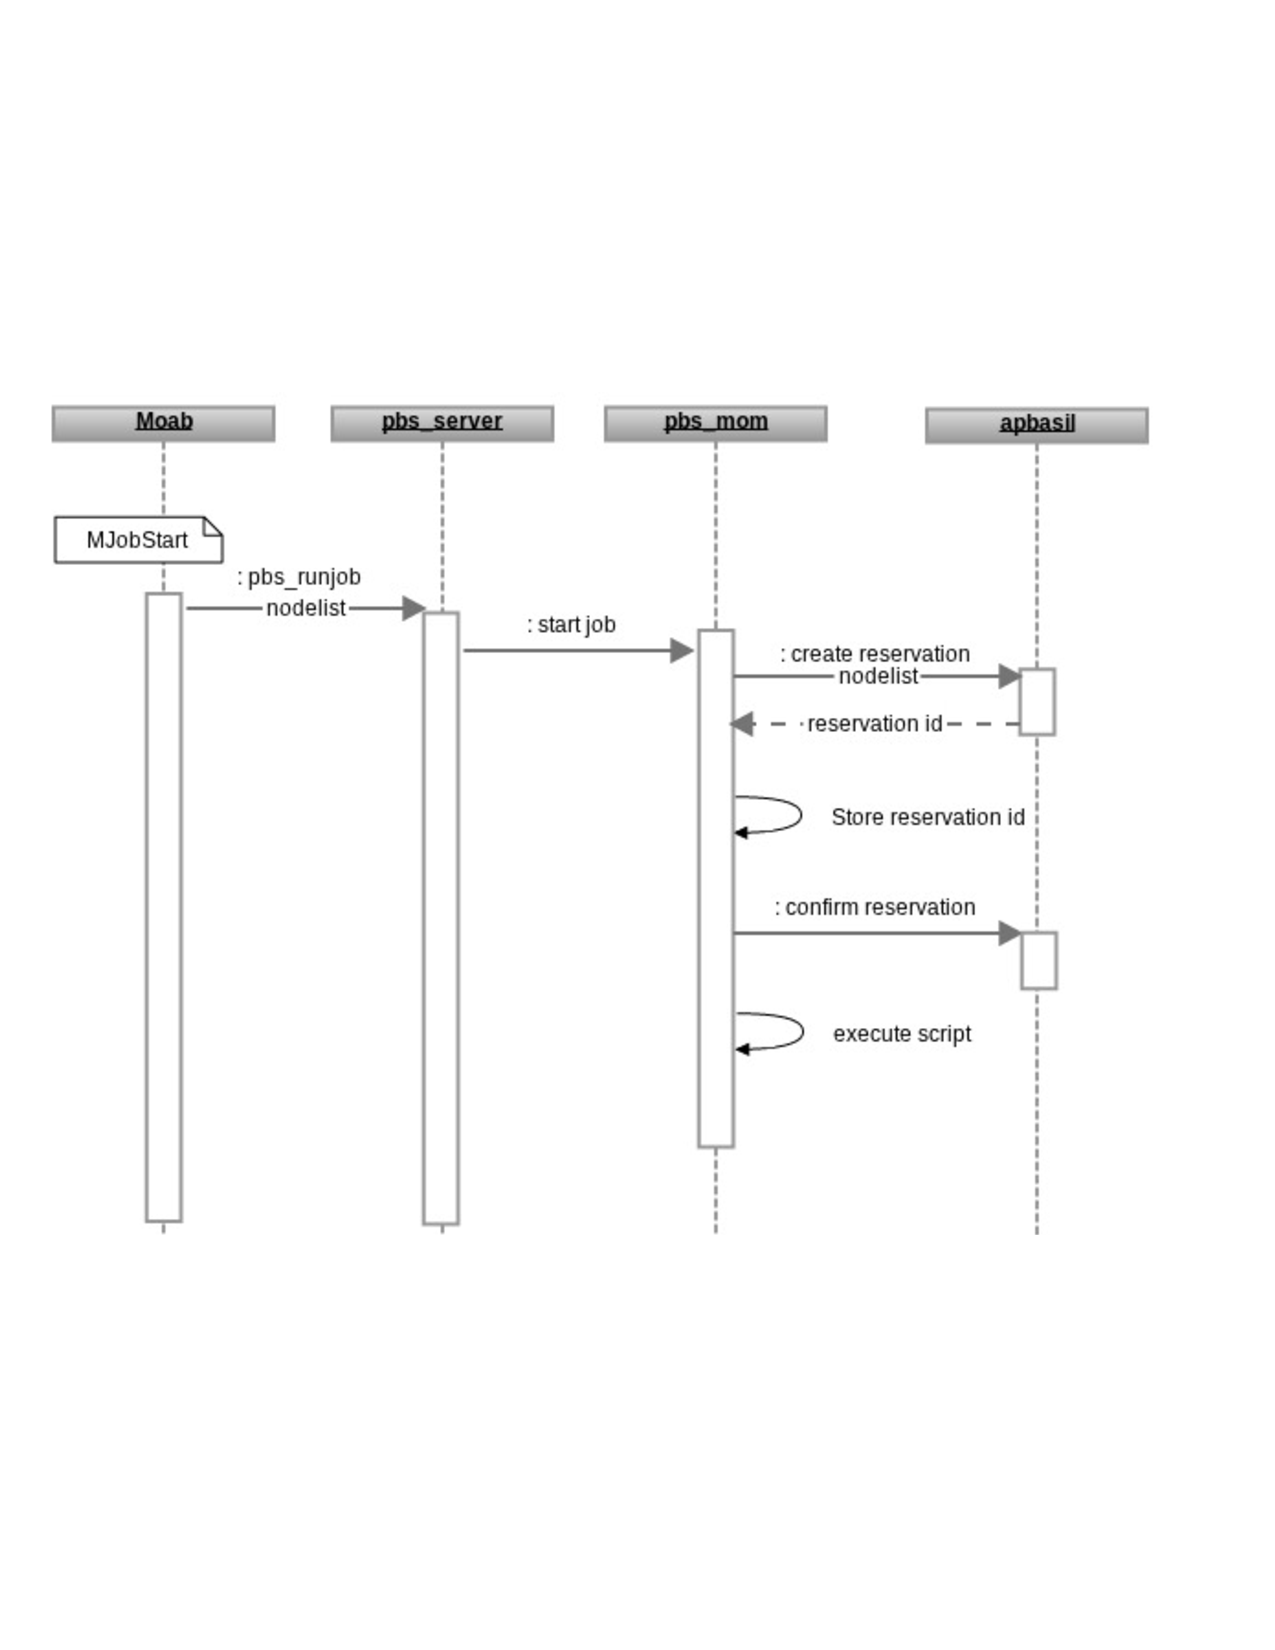
\includegraphics[width=3.5in]{figures/job-start.pdf}
  \caption{Job Starting}\label{fig:starting}
\end{figure}

\subsection{Advantages}

The new design simplifies configuration. No special binaries for Moab, TORQUE's
server or mom daemons are required, not even for the distinct types of mom
daemons. Less configuration makes for easier setup.

The whole model inherits superior support from Moab because from Moab's
perspective, scheduling the Cray is the same as scheduling any other cluster,
and it is no longer a one-off. Additionally, the code path that was used for
parsing output from the scripts in significantly slower than the code path for
interfacing with TORQUE for two reasons: text parsing happens faster and the
interaction is now through an API instead of a fork/pipe model.

Moab and pbs_server can now be moved outside of the Cray, allowing a number of
benefits. You can install them on as powerful of nodes as you like, and aren't
bound to whatever you have already.  If, after having the machine for a while,
you decide you need to upgrade the server and scheduler nodes then you can do
this without upgrading the entire machine. This also gives you back whatever
resources on the Cray Moab and pbs_server were occupying.

